\documentclass[12pt,a4paper]{article}
\usepackage{float}
\usepackage{commons/course}


%\hidesolutions

\شروع{نوشتار}

\سربرگ{تمرین اول}{}{ شمارش،مقدمات احتمال،احتمال شرطی،استقلال}{گردآورندگان: محمدرضا احمدخانی، سروش تسلیمی، علیرضا اکبری}


\section*{
شمارش و مقدمات احتمال
}

\مسئله{‌مجموعه بازی*}

تعداد زیرمجموعه های k عضوی از مجموعه ی $\{1, 2, 3, ..., n\}$ را بیابید که هیچ دو عضوی از آن متوالی نباشند.


\مسئله{‌رنگ بازی*}
در یک جعبه m توپ قرمز و n توپ آبی داریم.در هر مرحله یک توپ را به تصادف از جعبه خارج میکنیم تا زمانی که در مجموع r توپ قرمز دیده باشیم. احتمال این که در مجموع k توپ از جعبه بیرون آورده باشیم چه قدر است؟ 


\مسئله{‌جرئت یا حقیقت؟}
فرض کنید متغیر تصادفی X از یک توزیع
$
Binomial(n, p)
$
می‌آید.
\subsection*{الف}
با فرض اینکه 
$
p < \alpha < 1
$
و استفاده از نابرابری چبیشف، یک کران بالا برای 
$
P(X \ge \alpha n)
$
بیابید.

\subsection*{ب}
مقدار کران بالا را برای 
$
p = \frac{1}{2}
$
و
$
\alpha = \frac{3}{4}
$ 
تعیین کنید.


\مسئله{‌جایگشت}
صورت کلی مسئله 

\subsection*{الف}
صورت بخش اول 

\subsection*{ب}
صورت بخش دوم 

\subsection*{ج}
صورت بخش سوم

\section*{
احتمال شرطی ، استقلال
}

\مسئله{‌بچه چیه؟}
ثابت کنید متغیرهای
$ X_1 $
, ... ,
$ X_n $
مستقلند اگر و تنها اگر تابع توزیع توام آن‌ها به شکل زیر قابل بیان باشد.
\begin{center}
	$f( x_1, x_2, ..., x_n ) = \prod_{i=1}^n g_i(x_i)$
\end{center}
$ g_i $
تابعی مثبت است.



\مسئله{‌فروشگاه قطعات ماشین*}
شش پسر و نه دختر میخواهند که در یک صف کنار یکدیگر قرار بگیرند. فرض کنید متغیر S برابر با تعداد مکانهایی باشد که یک پسر و یک دختر کنار هم قرار گرفته باشند( به طور مثال در صف GBGGBBGBBGGGBGG متغیر S برابر با 8 است.)
مقدار میانگین S ( اگر تمامی ترتیب های قرار گیری این پانزده نفر را در نظر بگیریم)  برابر با چه مقداری است ؟




\مسئله{‌توپ بازی*}
\textbf{جدول
\lr{t}
در ادامه آمده است.}

اداره هواشناسی یک شهر، ۴ دستگاه سنجش آلودگی هوا را در یک منطقه قرار داده است. فرض کنید شاخص آلودگی هوا در این منطقه ثابت است اما این دستگاه‌ها دقیق نیستند و شاخص را با کمی نویز گزارش می‌دهند. در یک روز نسبتا آلوده، مقادیر گزارش شده توسط این ۴ دستگاه به شرح زیر است.
$$152, 148, 153, 153$$

\subsection*{الف}
با کمک داده‌های جمع آوری شده، یک بازه اطمینان ۹۵ درصد برای شاخص آلودگی هوا در آن ایستگاه ارائه دهید.

\subsection*{ب}
در صورتی که شاخص آلودگی هوا از ۱۵۰ بیشتر باشد، هوا در شرایط ناسالم برای تمامی گروه‌ها قرار می‌گیرد. عده‌ای از دانشمندان معتقدند که میانگین شاخص آلودگی ۱۵۰ بوده بنابراین هوای این منطقه ناسالم نیست، در حالی که عده‌ی دیگری معتقند میانگین شاخص آلودگی به طور معنی‌داری از ۱۵۰ بیشتر بوده و هوا ناسالم است. برای بررسی این افراد یک آزمون فرض طراحی کنید. فرض صفر و فرض دیگر این آزمون را بیان کرده و سپس مشخص کنید آیا با سطح اهمیت 
$0.05$
می‌توان فرض صفر را رد کرد یا خیر.

\subsection*{پ}
برای کاهش خطای نوع اول، باید سطح اهمیت را افزایش دهیم یا کاهش؟ برای کاهش خطای نوع دوم چه طور؟

\begin{figure}[H]
    \centering
    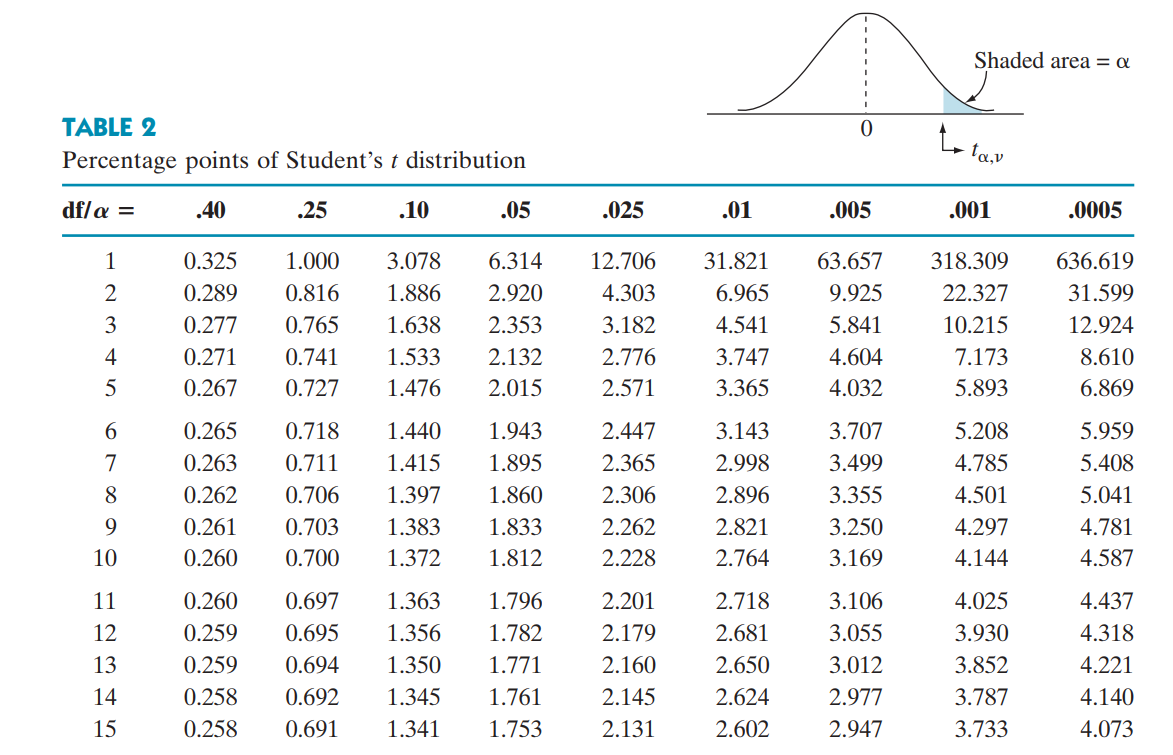
\includegraphics[width=7in,height = 5in]{tStudent}
\end{figure}



\مسئله{‌بادکنک بازی}
متغیر تصادفی 
$N$
تعداد تخم مرغ های یک مزرعه است که از توزیع پوآسون با متغیر 
$\lambda$
پیروی می‌کند. هر تخم مرغ با احتمال
$p$
به جوجه تبدیل می‌شود و شکستن تخم مرغ ها از هم مستقل است . متغیر تصادفی 
$X$ 
تعداد تخم مرغ هایی هستند که به جوجه تبدیل می‌شوند و متغیر تصادفی
$Y$
 تعداد آنهایی است که تبدیل نمی‌شوند . توزیع توام را برای دو متغیر تصادفی  
$X$ و $Y$
 بدست آورید. 






\مسئله{‌سکه بازی*}
دو نفر به نام‌های A و B مشغول یک بازی هستند که شرح آن در ادامه می‌آید. ابتدا A عدد 1 یا 2 را روی یک کاغذ می‌نویسد و آن را پنهان می‌کند. B باید حدس بزند عددی که A نوشته، چه بوده است. اگر عددی که A نوشته $i$ باشد و حدس B هم درست باشد، در آن صورت A باید $i$ تومن به B بدهد. اما اگر حدس B نادرست باشد، B باید $\frac{3}{4}$ تومن به A بدهد.\\
اگر B به صورت رندوم حدس بزند به طوری که با احتمال $p$ حدس بزند 1 و با احتمال $1-p$ حدس بزند 2، امید ریاضی پول دریافتی توسط B را در دو حالت زیر محاسبه کنید.

\subsection*{الف}
اگر A عدد 1 را روی کاغذ نوشته باشد.

\subsection*{ب}
اگر A عدد 2 را روی کاغذ نوشته باشد.

\subsection*{ج}
محاسبه کنید که به ازای چه مقداری از $p$، مینیموم امید ریاضی محاسبه شده در دو حالت بالا، ماکسیموم می‌شود.



\مسئله{
این کارا آخر عاقبت نداره!
\پاورقی{
Gambler's Ruin
}
(
برای علاقه‌مندان
)
}


در هر مورد تابع توزیع خواسته شده را به دست آورید و سپس تحقیق کنید متغیر تصادفی مورد نظر از چه خانواده ای از توزیع هاست. و با استفاده از آن امید ریاضی و واریانس توزیع را به دست آورید.
\subsection*{الف}
فرض کنید متغیر تصادفی $X$ از توزیع پارتو با متغیر $\theta > 0$ پیروی می کند که تابع توزیع آن به صورت زیر است:
$$f_{X}(x) = \frac{\theta}{x ^ {\theta + 1}} \quad x > 1$$
حال اگر متغیر تصادفی $Y$ به صورت زیر به دست بیاید، $Y$ از چه توزیعی پیروی می کند؟
$$ Y = \ln X$$

\subsection*{ب}
فرض کنید $Y$ متغیر تصادفی با توزیع نرمال استاندارد باشد. یعنی $Y \sim exponential(\lambda)$. حال اگر متغیر تصادفی $W$ به صورت زیر به دست بیاید، تابع توزیع آن را به دست بیاورید.$W$ از چه توزیعی پیروی می کند؟

$$W = \sqrt{Y}$$
\subsection*{ج}
فرض کنید $Z$ متغیر تصادفی با توزیع نرمال استاندارد باشد یعنی $Z \sim N(0, 1)$ . حال اگر متغیر تصادفی $Y$ به صورت زیر به دست بیاید، تابع توزیع آن را به دست بیاورید.$Y$ از چه توزیعی پیروی می کند؟
$$Z = e ^ Z$$
\subsection*{د}
فرض کنید $Z$ متغیر تصادفی با توزیع نرمال استاندارد باشد یعنی $Z \sim N(0, 1)$ . حال اگر متغیر تصادفی $X$ به صورت زیر به دست بیاید، تابع توزیع آن را به دست بیاورید.$X$ از چه توزیعی پیروی می کند؟
$$X = Z ^ 2 $$






\begin{flushleft}
	موفق باشید :)
\end{flushleft}



\پایان{نوشتار}
